\subsection{The user interface must be obvious and familiar}

The system can display the data in a precise, optimized, fully customized way. It can offer the user
the possibility to improve their life considerably. However, if we do not provide a user friendly experience, all our efforts will be in vain.
The user should feel that the system offers information in a fluid, intuitive, direct, straightforward manner and with
a logical sequence.
  
This logical sequence will allow the user the possibility of doing further investigating by themselves.

We look for simplicity in representing the information, we will avoid unnecessary ornamentation. Remember that less is more. A complicated design, with too many colors and too many different abstract shapes will be more difficult to interpret.

The representation must be unambiguous. We must not show information that is deceptive, or that requires time wasted in interpreting. When representing the information, we will 
include only what is truly necessary, always avoiding ornate graphics that only contribute noise to the representation.

We will seek to evoke familiarity, so that the user can quickly understand the structures used,
and therefore the minimum possible learning time is required.

In addition, in the wider world, there are several standards to which the user is already accustomed.
For example a magnifying glass is a familiar symbol for searching. If we use this icon, the user will quickly know what
function that performs, so it makes no sense to design a brand new icon.
It is important to give the user a degree of flexibility, that is, to enable them to make their own selections to be find the data that interests them.

When we speak of fluidity, we refer to user-system interactions.It is important that interactions
be like a two-way conversation, where we ask and let them know we are listening and responding. When the user
requires information from the system, they receive an indication that their request is being processed, and within no more than five seconds, an answer will be provided.
    
\subsubsection*{Suggested strategies} 

We must analyze carefully what information we want to presentaccording to our objetive. We will make a clear design, where all the elements are easy to recognize.
The structure will entail a logical sequence, as if it were a narrative history.
Each action that the user perform, must be clearly acknowledged (eg by some change in a button, or a spinning wheel icon) results must be delivered in less than five seconds.
We will steer clear of complicated representations, we will aim for familiarity and intuitiveness.
For example, if a calendar is used for the selection of dates, it doesn't make sense to use an hourglass, this will just be confusing forthe user.
Offer flexibility, the user must be able to interact with the interface and choose what they want to see.

\subsubsection*{In the context of Aire Guru \ldots}

Our tool uses an interpretation of Google's Material Design, which is very clean, without borders or decorations.
We chose a range of blue shades in combination with white and gray to evoke a relaxed atmosphere.
Importantly, we've taken care that all text has a good level of contrast with the background, so that it is easy to read.

The graphics have been designed in 2D, since they are easier to interpret and we lack the ambiguity that can occur when using depth as a measure.

The workflow of the different sections of Aire Guru is thought about in detail.
Aire Guru consists of different sections. By selecting a point on the map, we
will show detailed information for this point. The next section filters the information according to the preferences of the user
and lastly, it shows the history of pollutants since 2018 and the history of the pollution to which the user has been
exposed.

It is expected that the user will be interested in the level of pollution to which they are exposed in real time. Therefore, for users
that are identified and agree to share their location, Air Guru will show the pollution directly at the point where they are.

\begin{figure}[ht]
    \centering
    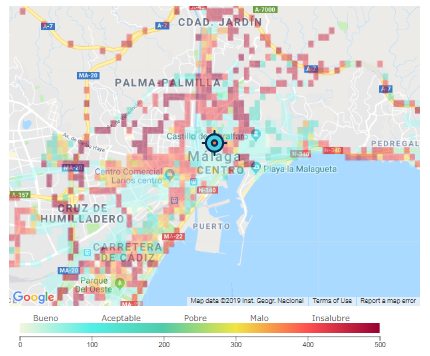
\includegraphics[width=12cm]{myLocation}
    \caption{My Location}
\end{figure}

Regarding flexibility, the user can see the state of the air pollution by dates. Intermediate filtering can be done both by medical conditions and by pollutants. Finally, in the lower area where we have
the historical data by area and personalization, we can visualize the information with different levels of detail; time, day, month and year. We can also
select the date we want.
\begin{figure}[ht]
    \centering
   \subfigure[Date filter]
    {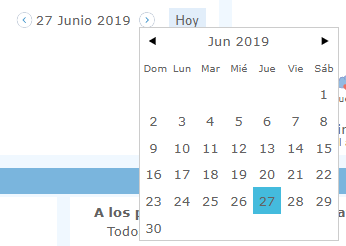
\includegraphics[width=5.5cm  ]{dateFilter}}
    \hfill
    \subfigure [Medical conditions filter]
       { \includegraphics[width=5.5cm]{MedicalConditionFilter}}
    \vfill
     \subfigure[Pollutans filter]
     { \centering 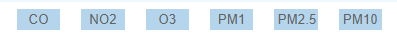
\includegraphics[width=6cm]{pollutantsFilter}}
  
  \caption{Filters}
    \end{figure}
    The same style, colors and iconography are used throughout the design so that the user can quickly become familiar with how it works, and can
    concentrate on the meaning of the data, rather than being distracted by trying to figure out what to do.
    
    Due to the large amount of data that is offered to the user, a waiting wheel has been implemented to indicate
    that the tool is processing information. Each time a control is pressed on the page, it is indicated with a change
    of color tonality. Also, progressive transitions are used, to indicate a process is happening.

    
    \begin{figure}[ht]
        \centering
       \subfigure[Searching bar]
        {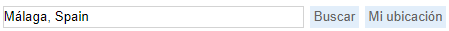
\includegraphics[width=5.5cm  ]{searchingBar}}
        \hfill
        \subfigure [Tabs]
           { 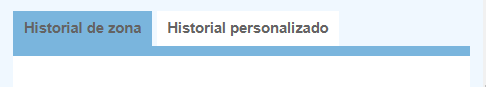
\includegraphics[width=5.5cm]{tabs}}
        \vfill
         \subfigure[Link]
         { 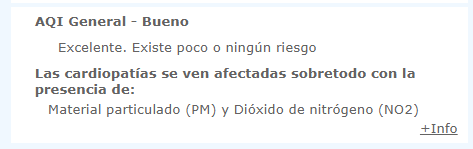
\includegraphics[width=6cm]{link}}
         \hfill
         \subfigure [Waiting symbol]
            { 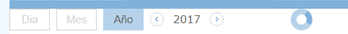
\includegraphics[width=5.5cm]{waitingSymbol}}
      
      \caption{Standard widgets}
        \end{figure}

        The elements that give us familiarity are the iconography that we use to show the AQI. We use clouds representing
             the air. The clouds are accompanied by a heart if the quality is good, by an exclamation mark if it is poor, by a cross if it is
             bad, and we change to a gas mask if the state is unhealthy.
            
             Today we are all familiar with GoogleMaps maps, so it makes sense to integrated this function.      

\subsubsection*{Evaluation}

\begin{itemize}
    \done Has a prevailing relaxed visual aesthetic.
    \done The representation follows a logical sequence.
    \done Familiarity - repetition of structures and representational colors create quick familiarity with the interface, and commonly used standard iconography is respected.
    \done Flexibility. The user can make multiple selections.
    \crossed Waiting times should be improved.
\end{itemize}